\documentclass{article}

% Language setting
% Replace `english' with e.g. `spanish' to change the document language
\usepackage[english]{babel}
\usepackage{ragged2e}
\usepackage{tabularx}
\usepackage{caption}
\usepackage{longtable}

\usepackage{lscape}

\usepackage{titlesec}

\setcounter{secnumdepth}{4}

\titleformat{\paragraph}
{\normalfont\normalsize\bfseries}{\theparagraph}{1em}{}
\titlespacing*{\paragraph}
{0pt}{3.25ex plus 1ex minus .2ex}{1.5ex plus .2ex}

% Set page size and margins
% Replace `letterpaper' with `a4paper' for UK/EU standard size
\usepackage[letterpaper,top=2cm,bottom=2cm,left=3cm,right=3cm,marginparwidth=1.75cm]{geometry}

% Useful packages
\usepackage{amsmath}
\usepackage{graphicx}
\usepackage[colorlinks=true, allcolors=blue]{hyperref}

\title{Physics for Sustainable Development in the Home: Using Criticality as a Measure}
\author{Meera Sheth \\ Supervisor: Dr George Giannopoulos}


\begin{document}

\maketitle




\begin{abstract}

In this project a methodology for estimating relative criticality was created to tackle the lack of consistency and comprehensive analysis of aggregation of indicators within available sustainability frameworks. This framework combines various indicators which reflect the supply risk, vulnerability and environmental concern surrounding the materials to provide a holistic overview of criticality. The application of this methodology on a case study determined the sustainability of using lithium-ion batteries for use with solar panels. Criticality scores were calculated for constituent materials, with copper, cobalt, lithium and nickel being of the highest criticality. Following the same methodology, criticality for recycled electric vehicle (EV) batteries were calculated to find there was a significant reduction in criticality compared to new lithium-ion batteries. This allowed the methodology to be applied to help provide a sustainable energy storage solution for domestic use. This framework encourages informed decision making in material selection, emphasising the importance of taking into account supply chain dynamics and environmental impact. Overall, this project delivers a systematic, data-driven approach to assessing material sustainability, with implications for design, manufacturing and even policy making. 

\end{abstract}

\newpage
\tableofcontents

\newpage

\section{Introduction}
Physics plays an important role in sustainable development since it can provide useful insights and core knowledge to tackle the world's most crucial and immediate challenges such as resource scarcity, climate change and tackling unsustainable practices. The United Nations Sustainable Development Goals outline some of these pressing issues and include plans on how to mitigate problems surrounding clean energy, industry and infrastructure and sustainable cities \cite{UNSDG}. Through the in-depth analysis of materials, their properties and factors effecting their extraction and use, sustainable development solutions can be achieved. 

\section{Material Criticality}

\subsection{What is criticality of materials?}

Criticality is the assessment of the risks connected with resource production, use and end of life \cite{graedel2014employing}. It is an evaluation of the importance of a resource to specific technologies, or industries on a global or regional level \cite{schrijvers2020review}. Graedel et al. (2019) defined criticality as ``the quality, state, or degree of being of the highest importance" \cite{graedel2019defining}. They also suggested that the most critical materials are those that require intensive processing to extract from parent ores, lack viable substitutes, have a low ability to be recycled and their transportation, manufacturing and storage requires high levels of energy. The time scale is also important to consider when assessing criticality since there may be different assessment conclusions when looking at the short, medium and long term trends \cite{riddle2015global}.

There are many aspects to consider when evaluating the criticality of a raw material, such as the geopolitical, social, and ecological effects on the extraction, production and use of the material \cite{kristof2010finalreport}. 
Many different methods to measure criticality have been developed by researchers, which consider the above factors. However, most studies have created a variety of `indicators' which assess the extent of how different drivers impact the supply risk of a material, have assigned a weighting to each indicator and provided the method of gathering and measuring this data \cite{achzet2013evaluate}. In one study which compared the different approaches, the indicators were reinterpreted to mean that `more' of the indicator meant a higher supply risk, which allowed easier comparisons to be made \cite{helbig2021overview}. In the study conducted by Achzet et al. (2013) \cite{achzet2013evaluate} and built on a few years later by Helbig et al. (2021) \cite{helbig2021overview}, it was identified that there were a few indicators which were popular amongst the different methods and were weighted highly in the overall assessments. The assessment of criticality of materials is a wide subject of debate and many different researchers have created their own methods of categorisation. These entail identifying the main drivers of criticality and analysing them to give a more holistic view of the impacts of the material over its lifetime. Many researchers also use it to rank the criticality of materials within a certain project or industry rather than define materials as critical or not critical. Criticality can be seen as a spectrum and is not just black and white. 

\subsection{Why is assessing criticality important?}

Assessing criticality is an important aspect of product design and helps inform decisions on material choice, leading to more sustainable actions being undertaken. Physics can play a major role in assessing criticality since analysis on material composition, properties and performance can help evaluate the status of materials. Insights into criticality help to identify and manage risks associated with the use of critical materials and allow strategies which aim to reduce their use to be implemented \cite{reller2011criticality}. 

Criticality assessments can be used to build resilience in the market to supply risks since it helps to identify them and evaluates the importance certain factors can have on the supply of a material and its impacts. 


\section{Methodologies}

There are many methodologies that researches have created to assess criticality. They can be categorised under 2 groups: supply risk assessment and vulnerability assessment \cite{gloser2015raw}, with many studies also including environmental concerns \cite{graedel2019defining}. Environmental concerns have been considered as the third group in this review. 

\subsection{Supply risk assessment}

Supply risk greatly impacts the criticality of materials since many resources are finite and non- renewable and the scarcity of the material correlates to how critical the material is. A supply risk assessment evaluates the factors which effect the supply rates of a material \cite{achzet2013evaluate}. There are many indicators that fall within this category such as depletion time, byproduct dependency, `substitutability', recyclability, and country concentration to name a few. Analysis and calculation of indicators are required to assess the impact on supply risk, for example, many researches calculate the Herfindahl- Hirschman Index (HHI) \cite{herfindahl1997concentration} to find the degree to which the supply of a material is concentrated in a handful of countries (country concentration). Some indicators are difficult to evaluate, such as byproduct dependency, since this relies on a whole new analysis of the host material- which could have a different evaluation. These indicators are relevant for sustainable development since they can provide useful information on the difficulty to obtain a material and its scarcity and if other materials are suitable and less critical. 

Some of the methodologies to evaluate supply risk are expert judgement, and scenario analysis using quantitative modelling \cite{schrijvers2020review}. It has been identified that there is a need to consider multiple perspectives to gauge a holistic view of supply risk. Expert judgement provides a good basis on which indicators will be useful to consider for a specific material, however this usually involves a more qualitative approach. Kolotzek et al. (2018) identified this to be a drawback and revised their assessment to remove expert judgement entirely and more heavily rely on quantitative methods \cite{KOLOTZEK2018566}. The emphasis on quantification is a good step towards gaining comparable data to find less critical substitutes, since it is difficult to apply a weight to a qualitative indicator to assess its contribution to the criticality of the material. 

Scenario analysis involves evaluating the different future scenarios that can occur and using these to assess the impacts on each version of events/ predictions. Ioannidou et al. (2019) identified that most methodologies were subject to fixed spatial and temporal referencing \cite{ioannidou2019future}, and hence creating a framework to predict multiple future scenarios was much needed since most studies created fixed outputs. A strength of this approach is that due to the difficult nature of accurately predicting trends, a variety of scenarios can be modelled and used as economic/ climate events unfold. 

\subsection{Vulnerability}

Vulnerability is the impact of a supply disruption of a specific resource \cite{schrijvers2020review, gloser2015raw, helbig2021selecting}. The impacts of a disruption in supply could be of economic and strategic importance e.g. a lack of a material could lead to shortages of products and backlogs of important resources.

Vulnerability is usually assessed by indicators which can be categorised into 3 sections: the first is assessing the demand for a resource in the general sense due to its use in multiple industries, the second is assessing the relative importance of the material compared to other materials which are used in the same system, and the third is the other indicators that can measure this such as substitutability, demand growth and import dependence \cite{schrijvers2020review}. Vulnerability is properly measured in terms of a product or industry due to materials having different levels of importance depending on their use.
    
Many researchers have used similar methods to assess vulnerability and this has also been in the form of appropriate indicators. Some popular indicators which are included in this category are: substitutability, future demand to supply ratio and value of products effected. 

Only one study (Graedel et al., 2012) evaluates vulnerability in multiple scopes such as on a national, technical and corporate level- with this being missing in many vulnerability studies \cite{helbig2016evaluate}. Many papers only focus on one at a time and fail to recognise that vulnerability differs when looking from an alternative point of view. 


\subsection{Environmental concerns}
Environmental concerns are some of the most important drivers when it comes to assessing criticality for materials and applying it for sustainable development. By understanding the impact natural disasters, recyclability and recycling potential have on the material during its life cycle, decisions on sustainable development can be made. Environmental implications may also be considered in this category such as the detrimental impacts due to the extraction or usage of the material \cite{gloser2014analyse}.

A key similarity in the measurement of all categories is that indicators are used throughout to measure influences and impacts. Some important indicators which represent environmental concerns are recyclability and recycling potential, resource depletion and biodiversity impact \cite{DAW2017173}. 

Some difficulties arise when trying to predict environmental concerns since these factors are very difficult to model and quantify \cite{schrijvers2020review}. There is not an agreed method to predict the environmental changes that will occur, especially as timescales for prediction increase.  


\subsection{Aggregation of indicators to calculate criticality scores}

The most important and frequently used methods of aggregation of indicators within supply risk, vulnerability and environmental concerns are \cite{frenzel2017raw}: 
\begin{itemize}
    \item Additive: the final score is calculated by summing the weighted/ scaled scores of the indicator values. These methods are used by Graedel et al. (2012) \cite{doi:10.1021/es203534z} and Panousi et al. (2016) \cite{panousi}. 
    \item Multiplicative: the final score is calculated by finding the product of weighted/ scaled scores of the indicator values. This method has been used for assessing the overall vulnerability of a material by the EU Commission \cite{entr2014report}.
    \item Mixed: The final score is a mixture of the sum and the product of indicator values e.g. by the EU Commission \cite{entr2014report}. 
\end{itemize}

The most popular methods identified to find the overall criticality score of a material are \cite{frenzel2017raw}:
\begin{itemize}
    \item Calculating the weighted sum of the scores given for each category.
    \item Determining the Euclidean distance of the point on the criticality plot (a material is plotted on a matrix depending on its supply risk and vulnerability). This method is adopted by Graedel et al. (2012) \cite{doi:10.1021/es203534z}, and can also include a third axis for environmental concerns \cite{nrc2008minerals}.
    \item Calculating the geometric mean of the categories. Using the geometric mean over the arithmetic mean is useful since the indicator values are not independent of one another. 
\end{itemize}

In order to find the aggregate score, many studies have normalised their quantitative metrics for easy comparison. Some studies have also normalised equivalent indicators in different studies to see if comparisons can be made between the approaches \cite{helbig2021overview}. 


\subsection{Limitations of methods}
Criticality has many well defined indicators which can be easily evaluated due to the presence and accessibility of data, however other indicators are much harder to quantify. This may be due to a lack of data, or because some factors are qualitative, meaning it is difficult to translate this into a numeric value. An important area of research is looking into methods to quantify these metrics in order to allow direct comparisons to be made.

Material criticality can also be reviewed in a number of different ways- it can focus on a specific material, a specific country in which it is imported/ exported and also can be focused around a certain product. This makes it hard for researchers to agree on a one size fits all approach to assessing material criticality. Some researchers also fail to collate indicators together depending on the same time scale. This can cause conflicting conclusions since some indicators may not be applicable to the scenario being considered.  

There is not a lot of agreement when it comes to categorising the indicators under supply risk and vulnerability, with many studies having much overlap between the two groups. This lack of consensus makes grouping indicators difficult for studies and makes it hard to differentiate between supply risk and its impacts. 

Some indicators are difficult to calculate due to the lack of availability of data. The data that is available is not necessarily taken with the idea of criticality assessments in mind and so some of what is needed is missing. This leads to researchers using proxy data that may not be the best choice \cite{schrijvers2020review}. Models can only be as good as the data that is input into them. Without the appropriate data, it is hard to create a model for each indicator. 

There is also a lack of thorough information on the aggregation of indicator scores, with many studies not including their methodology on the aggregation of scores to find the overall criticality. This makes it difficult to compare criticality scores for a given material, since there are a range of conflicting assessment results. Without adequate outlines on their approach, such as weightings, aggregation, data collected and used, it is difficult to draw conclusions based on others work. 



\section{Part 1: Construction of the Framework to Measure Criticality}

\subsection{Methodology}

In this project, the main aim was to adapt an existing methodology to measure criticality in order to factor in indicators which have not been quantified and included in the past. Using the findings from the literature review, the best methods from popular studies were extracted and reconfigured to be included within this new framework. Different studies had different strengths e.g. Helbig et al. (2021) \cite{helbig2021overview} were great at specifying appropriate normalisation, whilst Graedel et al. (2012) \cite{graedel2019defining} suggested a good approach to aggregate all indicator values using a criticality matrix. The weighted sum of the indicators within each category will be calculated to give category scores as well as overall criticality scores. To visualise the contribution of each, the scores can be then plotted as a 3D criticality matrix. The contribution of this aggregation of indicators is that the methodological steps are easy to follow and can be applied to evaluate a range of materials and case studies. This framework provides a toolkit to quantitatively and holistically assess criticality. 

\subsection{How are indicators selected?}

First the indicators which are used to measure criticality needed to be selected. From the literature review, the most popular indicators from 88 studies were identified to be included in this framework. Indicators which have been used more than 3 times within the studies researched were included \cite{helbig2021overview}, since it shows that it is an important factor to consider. However, these indicators were not robust when it came to measurable quantities for measuring the environmental concern category within criticality, so more research was conducted to find quantitative metrics which could be used to determine the environmental impact of the material. This led to an additional less popular indicator being added into this framework- $CO_{2}$ emissions throughout the materials extraction. This proved to be a measurable quantity and also allowed the environmental impact to be quantified and included within the overall assessment. 

The indicators chosen were then categorised into 3 criteria which are used to plot the value on the criticality matrix \cite{nrc2008minerals}. The 3 criteria are supply risk, vulnerability and environmental concern. The indicators are also carefully constructed so that the higher the value assigned to each indicator, the more it adds to the criticality of the material. This allows for consistency in the calculation of the overall criticality. The list of chosen indicators, along with the category assignment can be seen in table 1. 

\subsection{How are the indicators weighted?}

Inspired by the methodology outlined by S. Kar and K. Jha (2020), the interdependence relationships of the indicators were found \cite{doi:10.1080/15623599.2020.1742637}. In their methodology, the weights for each indicator were first decided using information gained from literature and experts, and then the weights given the interdependence relationships were calculated. These 2 weights were multiplied together to find the final weight. However, in this methodology only the weights from the interdependence relationship will be used since the first step involves a qualitative approach to determine the weights instead of quantitative. These relationships can be seen in figure 1. This identified the most important and influential indicators (the ones with the most inter-dependencies) and ones that did not link to many other indicators. Using this information, the appropriate weight is assigned to each of the indicators- the ones with the most inter-dependencies being weighted the most. The number of relationships for each indicator over the total number of relationships summed from each indicator is the weight assigned. For example, the scarcity indicator is weighted at 7/46 because it has 7 links to other indicators and the total links for all indicators sums to 46. The weights given to each indicator can be seen in table 1. This method allows for appropriate weightings to be allocated and allows a more quantitative approach to be taken as compared to other studies, where the calculations for the weighting were not detailed or even mentioned. This weighting can also be changed if the interdependence is found to be different for other (specific) cases, meaning it can be adapted to suit all scenarios, however it is unlikely that the interdependence will vary drastically. Criticality scores for the separate categories can also be found by calculating the weighted average of just the indicators within a single category. These intermediary scores allows conclusions to be made on the impact of the different groups of indicators. 

\begin{figure}[hbt!]
    \centering
    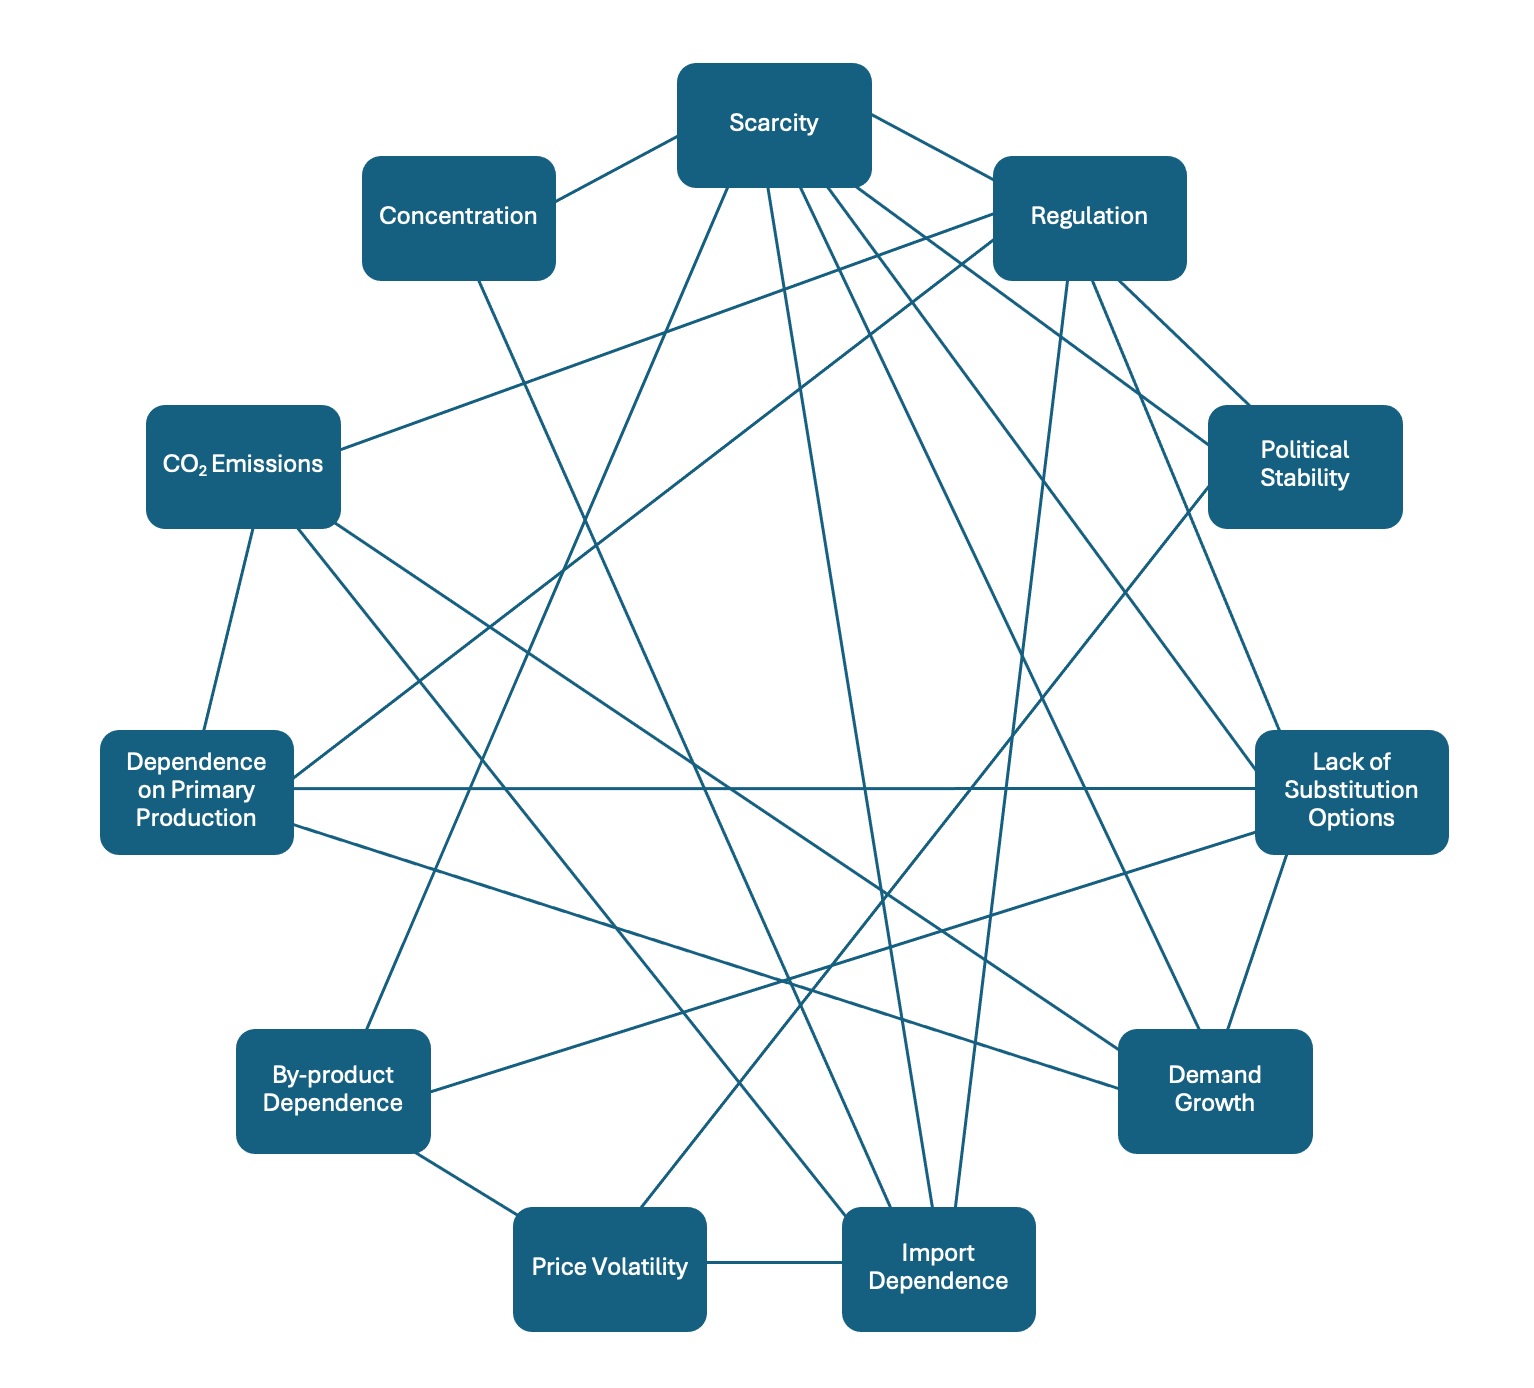
\includegraphics[width=0.7\linewidth]{Screenshot 2024-03-17 at 15.37.48.png}
    \caption{Interdependence relationships used to calculate the weighting of each indicator. The number of connections each indicator has is its weight and the sum of the number of connections for every indicator is the total weight.}
    \label{fig:Figure 1}
\end{figure}


\begin{longtable}{| p{.35\textwidth} | p{.25\textwidth} | p{0.1\textwidth }|} 
\hline

Indicator & Category & Weighting\\\hline
{Scarcity} & {Supply risk} & {6/46} \\\hline
{By-product dependence} & {Supply risk} & {3/46} \\\hline
{Concentration} & {Supply risk} & {2/46} \\\hline
{Political instability} &{Supply risk} & {2/46} \\\hline

{Regulation} & {Vulnerability} & {5/46} \\\hline
{Import dependence} & {Vulnerability}&{4/46} \\\hline
{Lack of Substitutions} & {Vulnerability} & {5/46} \\\hline
{Price volatility} & {Vulnerability} & {3/46} \\\hline
{Demand growth} & {Vulnerability} & {2/46} \\\hline

{Dependence on primary production} & {Environmental concern} & {4/46} \\\hline
{$CO_{2}$ emissions for life cycle} &  {Environmental concern} & {2/46} \\\hline

    \caption{Indicator classification and weighting for final criticality calculation.}
    \label{fig:Figure 1}

\end{longtable}

\subsection{Indicators}
In this section, descriptions of what the indicators measure will be given and the formulae needed for calculating and normalising them. One important criteria imposed on all indicators is that ``more" of the indicator equates to a higher score which increases the materials criticality. This is done to create a consistency within the framework and allow for fairer indicator aggregation to calculate the overall criticality score.

\subsubsection{Scarcity}

Scarcity is measured using depletion time (DT). Depletion for non-renewable resources is the ``quantitative and qualitative deterioration of mineral reserves, resulting in their scarcity" \cite{su13020862}. For other materials, this is the product of ``excess of resource consumption over its reproduction (physical depletion)" \cite{SANTOPIETRO199839}. This indicator is used to determine the number of years it will take to run out of this resource and its reserves. This has a major impact on supply risk and scarcity has many inter- dependencies with other indicators, meaning that long or short depletion times have an effect on its associated indicators e.g. the need to find substitution options. Depletion rate can be calculated using equation \ref{eq:1} and is measured in years. This calculation is a useful proxy for the determining the value. In order to use this within the criticality framework the normalisation given in equation \ref{eq:2} is applied \cite{doi:10.1021/es203534z}. This normalisation assigns a supply risk score of 0 for a depletion time of 100 years or above and a supply risk score of 1 to a depletion time of 0.


\begin{equation} \label{eq:1}
DT = \frac{\text{Reserve volume}}{\text{Rate of primary production}}
\end{equation}

\begin{equation} \label{eq:2}
DT_{normalised} = \left\{\begin{matrix} 0 \text{ if DT $>$ 100}
\\\frac{1}{100} (100\text{-}0.2(DT)\text{-}(0.008)DT^2) \text{, otherwise}

\end{matrix}\right.
\end{equation}

\subsubsection{By-product dependence}

This indicator measures the percentage of a metal that is mined/ found/ extracted as a by-product \cite{graedel2014employing}. This includes how much of the material is extracted from mined ores. GRANTA Selector can be used to find this data. Within the context of the framework, the higher the percentage, the lower the supply risk and hence a correction in the formula is needed. The normalised value for by-product dependence (BPD) can be calculated using equation \ref{eq:3}. 

\begin{equation} \label{eq:3}
BPD_{normalised} = 1 - \frac{BPD}{100}
\end{equation}

\subsubsection{Concentration}

Concentration is a measure of the sum of the square of the market share of each country. This tells us how many countries supply the material and if there is a large or small number of sources. The closer the normalised score is to 0, the higher the number of countries supplying the material, and hence a lower supply risk, since there are many sources. The higher the value is to one, the more a single country has a monopoly on the export of the resource, which increases the supply risk. HHI \cite{herfindahl1997concentration} is a measure of concentration and can be calculated using equation \ref{eq:4}. 

\begin{equation} \label{eq:4}
HHI = \sum_{n=1}^{N} s_{n}^2 
\end{equation}

The normalisation factor in equation \ref{eq:5}  \cite{doi:10.1021/es203534z} is applied to the HHI value from above. With this normalisation, an HHI value of 10,000 is translated to 1, the highest score.

\begin{equation} \label{eq:5}
HHI_{normalised}=\frac{1}{100} 17.5 ln(HHI) \text{-} 61.18
\end{equation}

\subsubsection{Political instability}

Political instability is measured using the World Governance Indicator (WGI): ``Political Stability and Absence of Violence/Terrorism" \cite{Worldbank}. This metric is updated annually by the World Bank and this score tells us how likely it is for the supply to be affected given the political dynamic of the country. Some of the factors which are incorporated into the metric are internal and external conflicts, terrorism, government stability and protests and riots. These can have major impacts on the supply chain and exporting/ importing schedules. WGI values range from 0 to 100 and so the normalisation used is given in equation \ref{eq:6}. This indicator focuses on the country which has the highest concentration of reserves (which can be determined when calculating the HHI), but can also be used to draw conclusions on the country in which it will be used.

\begin{equation} \label{eq:6}
WGI_{normalised} = \frac{WGI}{100}
\end{equation}

\subsubsection{Regulation}

This indicator can be measured using the average of many different indices: PPI (policy perception index), EPI (environmental performance index) and HDI (human development indicator). These indices give a more holistic understanding of criticality when applied in the context of the country which is the main supplier of that material. 

The PPI looks into the influence of policies on the mining activities in the country/ region of interest and this data is provided by the Fraser Institute. It takes into account factors such as overbearing regulations, regulatory duplication, how regulation is administered and taxation levels \cite{fraserinstitute}. Equation \ref{eq:7} shows the normalisation used for this index. 

\begin{equation} \label{eq:7}
PPI_{normalised} = \frac{1}{100}(100-PPI)
\end{equation}

The EPI evaluates the ability of a country/ region to cope with environmental concerns and is provided by the University of Yale. The index accounts for climate change performance, environmental health, and ecosystem vitality \cite{EPI}. Equation \ref{eq:8} shows the normalisation used for this index. In this framework, he higher the EPI, the better the country is equipped to deal with environmental concerns and keep the supply chains running smoothly \cite{jasinski2018assessing}. There is much conflict amongst different researchers on how to interpret this metric however. Roelich et al. (2014) had explained that this metric adds to the supply risk instead of reducing it since a better standard of environmental regulation could also mean that that mining activities could be blocked \cite{roelich2014assessing}.

\begin{equation} \label{eq:8}
EPI_{normalised} = \frac{1}{100}(100 - EPI)
\end{equation}

The final index, HDI, evaluates life expectancy, standard of education and standard of living of that country and is measured by the UNDP \cite{conceiccao2020human}. HDI is a score between 0 and 1, so it needs no normalisation. 

Overall, these indices give a holistic view of the impact of regulations on the supply of a material by incorporating different external influences. The average of all these scores gives the overall indicator score.

\subsubsection{Import dependence}

This will be focusing on a national perspective of the country in which it is being used. Net import reliance identifies how much control domestic policy has on the supply chain. A high import dependence means that the material is more vulnerable to supply risk. Import dependence can be calculated using equation \ref{eq:9}.

\begin{equation} \label{eq:9}
Net \text{ }Import \text{ }Dependence = \frac{Imports-Exports}{Domestic \text{ }Production+Imports-Exports}
\end{equation}

\subsubsection{Lack of substitutions} 

This is a measure of if there are viable substitution options. The higher the score, the fewer the number of options and hence the higher the vulnerability. This information is available on EduPack and is presented as a list of uses of the material, the percentage of each use which has substitutions and if the substitutes are of a poor, adequate or good quality. The higher the percentage of substitutes which are ``poor" or lacking, the higher the indicator value. The normalisation for this is presented in \ref{eq:11}, where ``sub" is the sum of the percentages where the substitutes are labelled as ``poor" or where there are no substitutions. 

\begin{equation} \label{eq:11}
sub_{normalised} = \frac{sub}{100}
\end{equation}


\subsubsection{Price volatility} 

This measures how the price fluctuates and how it can cause vulnerability. A higher price means less of the material can be imported causing shortages in supply. A step-wise normalisation is used to relate price volatility to an overall indicator score. The score increases in even increments every 100\% wide intervals in volatility up until 300\% \cite{goddin2019identifying}. Values for the volatility can be obtained from EduPack.

\begin{equation}
vol_{normalised} =  \left\{\begin{matrix}
0.6 \text{ if} \leq vol \leq 150 & \\ 
0.75 \text{ if } 150 <  vol \leq 250  & \\ 
0.9 \text{ if }250 < vol < 300 & \\ 
1 \text{ if }vol \geq 300 & 
\end{matrix}\right.
\end{equation}

\subsubsection{Demand growth}

This indicator looks at the increase in demand from 2022 to 2050. This information is given as a percentage and can be gathered from Statista. A stepwise normalisation is used to gather the score assigned to the material. 

\begin{equation} growth_{normalised} =  \left\{\begin{matrix}
0.4 \text{ if 0 }  \leq growth \leq 50 & \\ 
0.6 \text{ if } 50 <  growth \leq 80  & \\ 
0.8 \text{ if }80 < growth < 150 & \\ 
1 \text{ if }growth \geq 150 & 
\end{matrix}\right.
\end{equation}

\subsubsection {Dependence on primary production}

This indicator is in place of the `recyclability' indicator seen in other studies. This indicator looks into the dependence on primary production (DPP) such as if the product can be reused from other places or must be mined/ extracted again. This is measured by the `recycled content ratio' (RCR) and this data can be gathered from the International Energy Agency. This indicator is important because recycled materials mean that materials can be utilised without additional mining which makes it easier to source and less environmentally harmful. A recycled content ratio of above 50\% contributes to no impact on supply risk \cite{bastein2014draft}. The normalisation for this is given using equation \ref{eq:10}.

\begin{equation} \label{eq:10}
DPP_{normalised} = \left\{\begin{matrix} 0 \text{ if RCR $>$ 50}
\\1-\frac{1}{50} \text{RCR} \text{ ,otherwise}

\end{matrix}\right.
\end{equation}

\subsubsection{CO$_{2}$ emissions from primary production/ extraction} 

This measures the emissions from activities within the extraction of the product including: mining and extraction. The initial plan was to include emissions throughout the life cycle of the product, however this data is difficult to find for all the different applications of a material. If data is available however, this would be a good alternative. Data for this indicator can be found directly on ANSYS EduPack and is given as kg of $CO_{2}$ per kg of material. Step-wise normalisation will be used to determine the overall score for this indicator, with the score increasing in even intervals. Many studies do not include this indicator, however it is a quantifiable metric which can be used to measure the impact the material has on the environment through emissions. By the inclusion of this indicator, more weighting can be applied to the environmental concern criteria so that it can have more of an influence in the overall criticality value. The normalisation of this indicator is best determined after data has been gathered for a group of materials which are of interest. This allows a criticality score to be assigned to the materials relative to each other. The data can be normalised by dividing the data for each material by the highest data value. 

\section{Part 2: The Battery Case Study}

\subsection{Background}

In the current economic climate, where many people are looking to reduce their high energy bills, renewable energy is becoming increasingly more attractive. Solar panels and battery energy storage is one of the alternative solutions people are turning to, which is encouraged by government schemes. For a 3-bedroom home, savings could be as much as £1190 per year \cite{solarsavings}. 

There are many benefits to using an in-house battery storage system especially when it is connected to a photovoltaic cell. The cost benefits to the consumer are one of the biggest advantages since it can encourage the transition to solar panel use. Another advantage is that generating electricity using solar panels reduces the dependence on the grid, which generates 33\% of its electricity using non-renewable methods \cite{renewableshare} such as burning fossil fuels. Making the switch to solar energy could also help achieve the UK governments goal of generating 95\% of its electricity using low-carbon sources \cite{renewableshare}. 

Solar energy is also a low emission solution, with the majority of its emissions taking place in the manufacturing of its batteries. Batteries are composed of a variety of critical materials and the majority of emissions released in a battery's lifetime come from manufacturing and disposal. Therefore it is important to investigate the sustainability of building batteries and how it can be improved by conducting a criticality study using the methodology detailed in the previous section. Some of the improvements can be making material substitutions or using more recycled materials. 

In this case study, the criticality of the constituents of the lithium-ion battery will be calculated and used to identify the most critical materials. From this, the criticality of employing a used EV battery will be compared to see if it is a more feasible option when it comes to improving sustainability. Adopting EV batteries is possible since even at their end of life, they retain 80\% of their initial capacity \cite{BAI2020304}- making it suitable for re-purposing. Reusing batteries as opposed to recycling them may be a better alternative since recycling processes that extract the rare-earth metal components from batteries such as pyrometallurgy and hydrometallurgy can be harmful to the environment \cite{sludge}. Pyrometallurgy involves high temperature smelting and is a highly energy intensive process. It creates a waste product called ``black mass" which is a sludge of various rare earth elements and other hazardous chemicals such as alkylfluorophosphates, which pose serious health concerns \cite{grutzke2015investigation}. Hydrometallurgy threatens natural habitats since it causes eutrophication and ozone depletion \cite{christensen2021risk}. 

The direct re-purposing of EV batteries as opposed to creating new ones or recycling old batteries may be a better energy solution. Knowing the criticality of constituent materials and the harm of recycling batteries will allow more informed decisions to be made and can encourage the reuse of old batteries.

\subsubsection{Which Battery is Best?}

There are many different types of batteries, all which differ in their characteristics. The most popular type of batteries are lead-acid, lithium-ion and nickel-cadmium. How can the most suitable battery be chosen for the intended case-study? Figure 2 shows the power density and energy density of multiple battery types. This graph created in GRANTA Selector shows that lithium-ion batteries provide the best ratio of energy and power density. From this it is evident why lithium-ion batteries are a popular choice for many systems. There are some requirements when it comes to deciding which battery is fit for the specific purpose of energy storage from solar panels for domestic use. Following on from figure 2, a series of filters were used to determine which battery type would be the best fit for the case study. The following criteria were applied and yielded results shown in figure 3. The battery needs to be rechargeable so that it can be charged during the day using solar panels and discharged in the evening as energy is used to light the house and run appliances. The cycle life needs to be relatively high (around 2000-6000 cycles) so that the battery can be used for many years to make it cost effective for the consumer. This is assuming a maximum of one cycle a day. An average home will need a battery energy capacity between 10kWh and 20kWh to fulfil their energy needs- however multiple batteries can be combined to achieve the wanted size and so this does not need to be one of the filters. A high energy density is also beneficial since it means that the battery can do work for a longer time relative to its size. This can allow less space to be taken up within the home to store the equipment. Figure 3 indicates that the batteries which pass the additional filters are LFP and NMC. 

Using this information, the framework to determine criticality can be applied to different lithium-ion batteries. 

\begin{figure}[hbt]
    \centering
    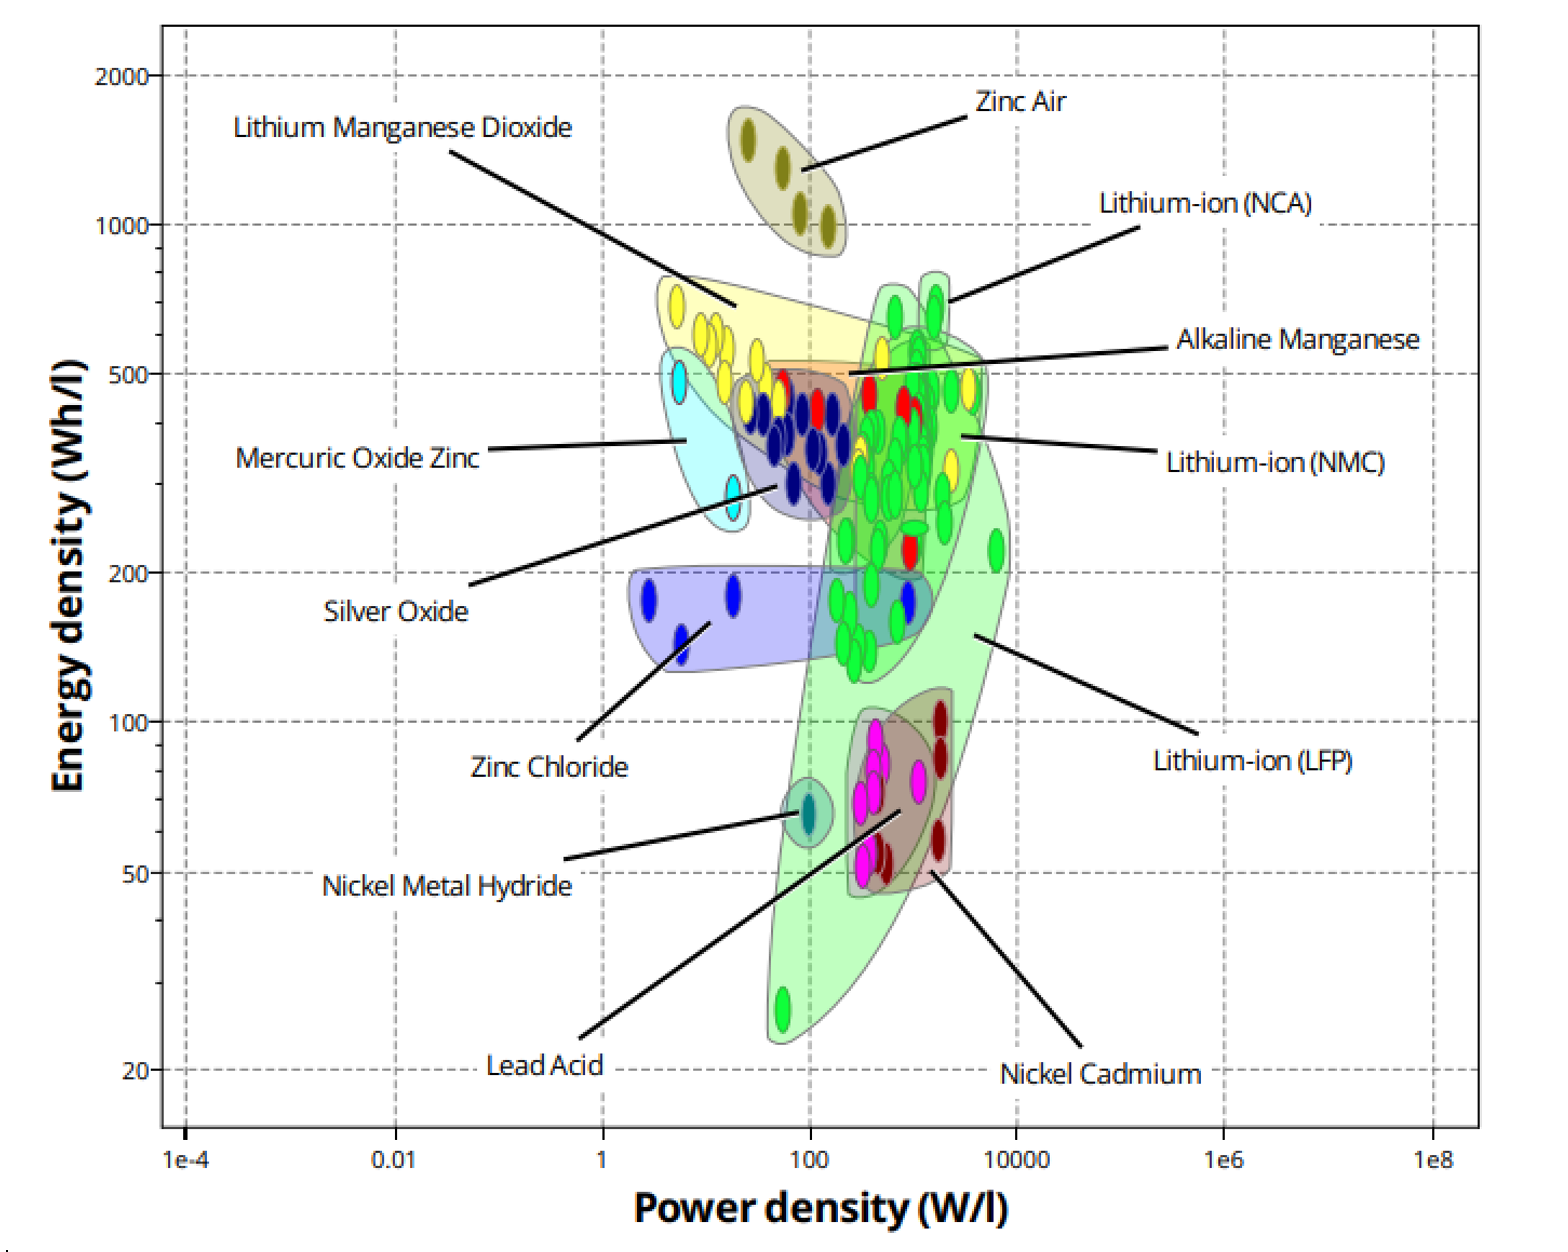
\includegraphics[width=1\linewidth]{Screenshot 2024-03-16 at 22.29.27.png}
    \caption{Ashby plot of all types of batteries displaying their power and energy density ranges. Each battery type has an envelope grouping them together to understand the range of values it can take.}
    \label{fig:2}
\end{figure}

\begin{figure}[hbt!]
    \centering
    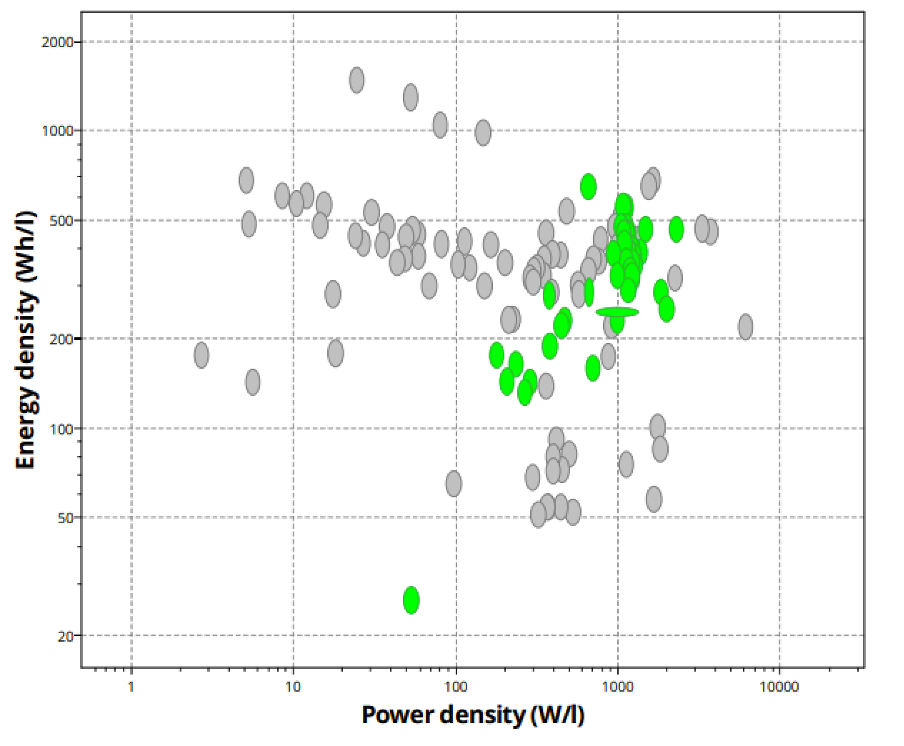
\includegraphics[width=1\linewidth]{filter graph.png}
    \caption{Graph to show the suitable battery types attained from applying filters. Filters include: ability to be rechargeable and a life cycle ranging between 2000 and 6000 cycles. These filters were applied to ensure the batteries were fit to be used within a solar panel energy storage system. Between 2000 and 6000 cycles are ideal so that the battery can be used for multiple years. LFP and NMC satisfied criteria.}
    \label{fig:3 }
\end{figure}


\subsection{Application of Framework}
\subsubsection{Standard Lithium-ion Batteries}

In the context of the case-study, the methodology to measure the criticality of the materials that make up different battery types was applied. The first step was finding out how each battery is divided up in terms of its material components. Table 2 shows the materials and the proportions of each within a battery. It is important to note that only the materials within the cathode have been listed since this is the portion of the battery where all the critical materials are located \cite{zou2013novel}. This allows for a narrower focus. After identifying the list of the most important metals used within the construction of a battery, the criticality was calculated using the methodology highlighted in section 4. Table 3 contains the scores for the supply risk, vulnerability and environmental concern as well as the aggregation of all to get the total criticality estimation.
\newpage
\begin{longtable}{| p{.15\textwidth} | p{.22\textwidth} | p{0.1\textwidth} |p{0.15\textwidth} |p{.1\textwidth} |p{.1\textwidth}|} 
\hline

Metal & $LiNi_{0.8}Co_{0.15}Al_{0.05}O_{2}$ cathode (\% of mass) \cite{gaines2011life}& $LiMn_{2}O_{4}$ cathode (\% of mass) \cite{gaines2011life}& 
$LiNiMnCoO_{2}$ cathode (\% of mass) \cite{batterycomp}& $LiCoO_{2}$ cathode (\% of mass) \cite{WANG2016204}& 
$LiFePO_{4}$ cathode (\% of mass) \cite{WANG2016204}\\\hline
{Aluminium} & {21.9 } &{21.7}& {22.72}& {5.2} &{6.5} \\\hline
{Cobalt} & {2.3}& {0.0}&{8.45}& {17.3}& {0.0}\\\hline
{Copper} &  {13.3}& {13.5}& {16.60}& {7.3}& {8.2}\\\hline
{Iron/Steel} &{0.1}& {0.1}& {8.79}& {16.5} &{43.2}\\\hline
{Lithium} &  {1.9} &{1.4} &{1.28} &{2.0} &{1.2} \\\hline
{Manganese} &  {0.0} &{10.7} &{5.86} &{0.0} &{0.0}\\\hline
{Nickel} &  {12.1} &{0.0} &{14.84} &{1.2} &{0.0}\\\hline

\caption{Constituents of lithium-ion battery cathodes given as a percentage of total mass.}
\end{longtable}

%reuslts table for criticality of metals:
\newpage
\begin{longtable}{| p{.15\textwidth} | p{.15\textwidth} | p{0.15\textwidth} |p{0.15\textwidth} |p{.15\textwidth} |}
\hline

Metal & Supply Risk Score & Vulnerability Score & 
Environmental Concern Score & Overall Criticality\\\hline
{Aluminium} & {0.392} &{0.336}& {0.079}& {0.309} \\\hline
{Cobalt} & {0.657}& {0.636}&{0.633}& {0.643}\\\hline
{Copper} &  {0.761}& {0.657}& {0.331}& {0.634}\\\hline
{Iron/Steel} &{0.574}& {0.579}& {0.014}& {0.479}\\\hline
{Lithium} &  {0.470} &{0.673} &{0.973} &{0.659} \\\hline
{Manganese} &  {0.560} &{0.713} &{0.346} &{0.599}\\\hline
{Nickel} &  {0.820} &{0.694} &{0.092} &{0.630}\\\hline

\caption{Criticality scores for various metals which make up popular lithium ion batteries.}
\end{longtable}

From table 3, it is clear that lithium, cobalt, copper and nickel are of the highest criticality from the application of this framework. It is also worth noting that lithium had the worst environmental impact of all the metals, yielding a score of 0.973 for environmental concern. This shows that relative to the other metals, lithium has the highest amount of carbon emissions and the lowest recycling rate, making it very unsustainable and a highly critical material. Cobalt scored consistently high in all 3 categories, whereas copper and nickel scored the most in the supply risk and vulnerability category. This shows that the criticality of these is mostly affected by the supply risk involved in obtaining the material and the impact of a disrupted supply chain. Due to the scope of the study being the UK, it was identified that the UK does not domestically produce many metals, with aluminium being the exception where a considerable amount is produced in the UK (see Appendix A). This shows that the majority of required metals need to be imported from other countries which effects the amount of $CO_{2}$ emitted due to transportation, leading to a higher score for net import dependence. Another notable indicator was dependence on primary production. Many metals were not fully recycled to their full potential even if they are critical metals. This suggests that recycling them could be more cost and energy intensive than sourcing them directly from natural resources. This is the case for lithium where recycling them from spent batteries can cause toxic chemicals to be released into the environment. 

The least critical metal was found to be aluminium which scored low in all 3 categories. Its abundant supply, high recycling rate and good regulation surrounding it allowed the criticality of this metal to be quite low. It scored the lowest in all 3 categories, with the exception of the environmental concern category, where iron scored lower. This was due to the fact that the recycling rate for iron was lower than aluminium, but the $CO_{2}$ emissions per kg were 5.6 times lower than aluminium. 

Using the information from table 3, the overall criticality of the cathode was calculated. This allows an average to be found for the entire product, allowing a better comparison to recycled EV batteries to compare and contrast the criticality and help inform choices on which is the more sustainable option.

Table 4 shows that the criticality of different lithium ion batteries are not all the same. Whilst some of the scores are higher than others, the overall criticality is similar. The score difference between the LMO (the lowest criticality battery) and the LCO (highest criticality battery) is 0.074. Whilst this may appear small in comparison, the difference is large enough to impact decision making processes with regard to sustainability. This difference is due to the varying proportions of metals within the cathode. Some batteries have a more conservative proportion of highly critical metals, such as the LFP battery, whereas others such as the NMC and LCO are more abundant of copper and cobalt. The overall criticality is relatively lower compared to the individual criticality of the materials assessed also due to this. The most critical materials such as lithium and cobalt do not make up a large portion of the battery and in fact are only needed in small quantities in all cases. It can be seen that the least critical battery types are the LMO ($LiMn_{2}O_{4}$), LFP ($LiFePO_{4}$) and NCA ($LiNi_{0.8}Co_{0.15}Al_{0.05}O_{2}$). From figure 3 it is evident that from these batteries, the battery that satisfies all criteria is the LFP battery. This battery has relatively low proportions of the highly critical materials such as lithium, cobalt and copper and fulfils the filter criteria detailed in section 5.1.1.

\newpage
\begin{longtable}{| p{.25\textwidth} | p{.25\textwidth} |}
\hline
Battery Type & Overall Criticality \\\hline

{$LiNi_{0.8}Co_{0.15}Al_{0.05}O_{2}$} &{0.497} \\\hline
{$LiMn_{2}O_{4}$} & {0.478}\\\hline
{$LiNiMnCoO_{2}$} &{0.521}\\\hline
{$LiCoO_{2}$} &{0.552}\\\hline
{$LiFePO_{4}$} &{0.486}\\\hline

\caption{Criticality scores for various metals which make up popular lithium ion batteries.}
\end{longtable}

\subsubsection{Idealistic Study of the Recycled EV Battery}

The same methodology outlined in section 4 can be used to estimate the criticality of using a recycled EV battery instead of a brand new lithium-ion battery. The data used within the calculations of indicators reflects an idealistic case where most of the spent EV batteries are repurposed and used for secondary reasons (such as an energy storage unit for solar power). The country specific indicators were refocused towards the UK because the case study is specific to using the spent EV batteries that are already within the country, which ultimately also reduces the carbon emissions of transportation. The depletion time was set to $``>100" $ because EV battery technology will be increasingly more popular due to the aim of achieving the 2-degree climate scenario. This value decreased the indicator score to 0 as detailed in the section 4.4.1. The recycled content ratio was set to $``>50"$ because this is the idealistic scenario and there is an assumption that a high enough percentage of EV batteries can be reused as an SLB (second-life battery). The CO$_{2}$ emissions were not based on the mining, extraction and processing of the battery, but instead the emissions associated with the relocation and implementation of the battery in its new purpose. Data for this was not readily available, but can be studied case by case and used within the framework to assess the criticality. Table 5 shows the results of the study. Figure 4 displays these results in a visual format to better understand the contributions of each category towards the final score. The environmental concern is particularly low for the EV battery since it does not need to be recycled to extract all the metals and can be straight away repurposed without extra processing. This is a better alternative to using a new battery since it doesn't require additional mining and importing. It scored even lower than the LFP which was the battery with the second lowest criticality which was fit for purpose. It is clear that using recycled EV batteries greatly reduces the criticality by over 79\%. This shows how desirable it is to reuse end of life EV batteries, especially since they are still at 75-80\% of their original capacity, making them perfect for energy storage within the home. However, their life cycle is decreased to between 1000 and 3000 cycles \cite{liu2022overview}. This does mean some EV batteries will not fulfil the criteria identified previously of having a minimum 2000 cycles remaining, but due to the lower overall criticality and the efficient reuse and re-purposing of batteries to utilise their full capacity, they still make a great solution for energy storage needs.

Another aspect to consider is that multiple batteries are required to provide the same energy storage capacities as the EV battery. Most commercial solar batteries are around 5-10kWh and hence the more batteries that are needed the more critical resources are needed to produce them. 


\begin{longtable}{| p{.21\textwidth} | p{.15\textwidth} | p{0.15\textwidth} |p{0.15\textwidth} |p{.15\textwidth} |}
\hline

{} & Supply Risk Score & Vulnerability Score & 
Environmental Concern Score & Overall Criticality\\\hline
{Recycled EV Battery} & {0.400} &
 {0.271} &
 {0.00}&
 {0.272}
 \\\hline

\caption{Criticality scores for the recycled EV battery case.}
\end{longtable}

\begin{figure}[hb]
    \centering
    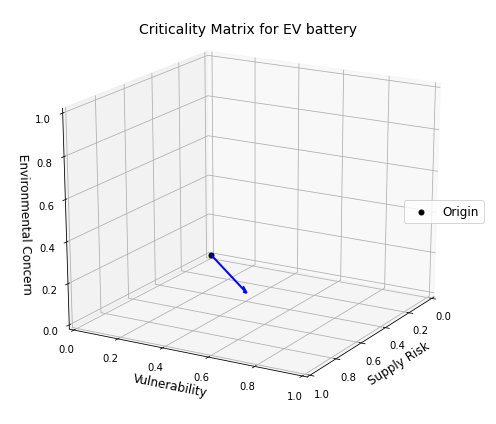
\includegraphics[width=0.6\linewidth]{crit matric EV battery.png}
    \caption{Criticality matrix to show the contributions of each category to the overall criticality of the EV battery. Environmental concern is 0 whereas the supply risk and vulnerability scores contribute most to the final value. The matrix proves to be an easy tool to visualise results.}
    \label{fig:enter-label}
\end{figure}

\section{Discussion} 

The aim of this project was to create a framework of estimating criticality which included quantification of methodology which had not been well defined previously and to use it to inform decisions on sustainability within the context of a case study. The case study chosen highlighted that the best alternative to new batteries is a recycled EV battery due to its low relative criticality, its large capacity (75-80\%) and its ability to be recharged. This evaluation consisted of many steps, such as identifying the materials of interest within the batteries, finding data to calculate the criticality, and using this alongside external requirements to decide upon a suitable battery choice. This framework allows changes in the supply chain, vulnerability and environmental concern to be taken into account. It calculates the relative criticality of materials compared to each other and the specific processes e.g. the amount of carbon emissions are specific to the choice of extraction and processing and this indicator has been constructed so that it compares the emissions to that of the highest emission value. This makes the overall criticality value specific to the scope of interest and doesn't necessarily mean that if the source of one of the materials is changed to one scoring lower on the regulations and political stability indicators, that the absolute criticality of the material goes up. It changes relative to the other source and hence the less risky supplier is a justified choice to obtain the material from. The data obtained for the indicators can be as specific or as general as needed e.g. the demand growth indicator can be interpreted to look solely into the projected demand growth for a particular technology or an entire industry depending on the focus of the study. This option of customisation allows a variety of scenarios to be tested and compared, ultimately leading to a well researched and justified choice of materials to be made. For example, if multiple sources were researched for each material instead of just the one country which had the highest concentration of that material, the criticality values would be different and perhaps another battery type would be the better choice.

\section{Conclusion}
During this project, methods of evaluating the sustainability were investigated to create a novel approach to estimating the relative criticality of materials. A reoccurring issue faced was the disagreement in the definition of criticality which meant that even using homogeneous indicators, the resulting criticality evaluations varied from study to study. This meant many studies had different evaluations of the same material making it difficult to choose the right methodology. Additionally a whole host of studies lacked detailed steps to recreate their framework and required further information on the aggregation of scores to prove to be repeatable. This inspired a criticality study to be undertaken to create a detailed methodology of estimating the criticality of a given material which was process and country specific allowing a more scenario-dependent criticality score to be attained.


In order to create this methodology, the most recurrent indicators from studies were chosen to be part of the evaluation so that a well-rounded view of criticality could be examined. The aim of this study was to help inform on the decision making process for materials, and by extension, objects in which the indicator information is available. From this, the application of this to a case study of a battery showed the methodology in use and the results garnered were used to decide upon the best choice. This study ultimately generates comparable metrics for materials, allowing a holistic insight into the criticality of a material and in turn, allows us to make judgements on the sustainability of the material depending on its source and use. Some drawbacks of the method are that it cannot measure criticality on an absolute scale, and cannot be of assistance in cases where that is required. The methodology can also be built on to examine the performance of the different batteries and materials within the use described. This can be done using ANSYS Fluent. It would be particularly useful to analyse battery health and thermal properties of the used EV battery to ensure there would be no overheating and verify overall safety. 

Overall, this methodology can be used consistently within projects to estimate the criticality of materials under specific scenarios and influence decision-making within the design phase, the final material selection and final product selection.

\bibliographystyle{unsrt}
\bibliography{name}
\newpage
\newgeometry{left=1.5cm,bottom=1.3cm}
\begin{landscape}
    \Huge 
    \appendix
\section{Raw Data for Indicator Calculations}

% Table generated by Excel2LaTeX from sheet 'Sheet1'
\begin{table}[htbp]
  \centering
  \scriptsize
    \begin{tabular}{lrrrrrrrrrrrlrrr}
          & \multicolumn{1}{l}{DT/ years} & \multicolumn{1}{l}{\%Mined} & \multicolumn{1}{l}{HHI} & \multicolumn{1}{l}{WGI} & \multicolumn{1}{l}{PPI} & \multicolumn{1}{l}{EPI} & \multicolumn{1}{l}{HDI} & \multicolumn{1}{l}{Imports/kg} & \multicolumn{1}{l}{Exports/kg} & \multicolumn{1}{l}{Dom prod/kg} & \multicolumn{1}{l}{No subs for \%} & Vol & \multicolumn{1}{l}{Dem growth 2050 /\%} & \multicolumn{1}{l}{RCR} & \multicolumn{1}{l}{$CO_2$ emissions (kg/kg)} \\
    Lithium & 1101.150 & 0.60  & 3417  & 81.60 & 77.73 & 60.1  & 0.951 & 2400000 & 1,469,830 & 0     & 13    & \multicolumn{1}{r}{136.0} & 491.0 & 5     & 79.60 \\
    Cobalt & 49.306 & 0.55  & 4839  & 6.13  & 21.30 & 36.9  & 0.479 & 548,178 & \textcolor[rgb]{ .2,  .2,  .2}{68,421} & 0     & 27    & \multicolumn{1}{r}{195.0} & 462.0 & 30    & 45.30 \\
    Nickel & 35.949 & 1.05  & 1541  & 73.58 & 70.19 & 50.0  & 0.936 & 884,243 & 24000 & 0     & 40    & \multicolumn{1}{r}{122.0} & 99.0  & 68    & 14.65 \\
    Cadmium & 3.122 & 0.20  & 1715  & 28.30 & 15.73 & 28.4  & 0.768 & 45134 & 27165 & 0     & 26    & \multicolumn{1}{r}{224.0} & 12.5  & 23    & 5.42 \\
    Aluminium & 469.460 & 32.00 & 1782  & 81.60 & 77.73 & 60.1  & 0.951 & 146,967	 & \textcolor[rgb]{ .2,  .2,  .2}{182,337} & 148800000 & 6     & \multicolumn{1}{r}{49.4} & 9.0   & 76    & 12.60 \\
    Iron/steel & 71.300 & 47.50 & 1969  & 81.60 & 77.73 & 60.1  & 0.951 & 7061000 & \textcolor[rgb]{ .2,  .2,  .2}{1,765,230} & 0     & 0     & \multicolumn{1}{r}{253.0} & 1.0   & 60    & 2.25 \\
    Copper & 37.297 & 2.65  & 1159  & 51.54 & 46.68 & 46.7  & 0.855 & 15252000 & 1,825,950 & 0     & 60    & \multicolumn{1}{r}{46.2} & 7.0   & 40    & 5.04 \\
    Manganese & 67.978 & 0.15  & 1560  & 19.81 & 29.65 & 37.2  & 0.713 & 4,717,100 & 698,173 & 0     & 92    & \multicolumn{1}{r}{170.0} & 4.0   & 37    & 4.88 \\
    EV battery  &       & 0.00  & 3570  & 28.30 & 71.00 & \textcolor[rgb]{ .133,  .133,  .133}{77.7} & 0.940 & 0     & 0     & 1000000 & 0     & <100  & 904.6 & 100   & 0.00 \\
    \end{tabular}%

      \caption{Raw data used within the methodology outlined in section 4 to calculate the criticality of the different constituents of lithium-ion batteries and the recycled EV battery for the case study. }
  \label{tab:addlabel}%
\end{table}%
    
\end{landscape}


\end{document}